\Chapter{MAGNIS (MAGnetized Negative Ion Source)}
\begin{refsection}

\chaptermark{Modèles plasmas froids magnétisés}

Dans ce chapitre, nous proposons un nouveau modèle fluide pour décrire le
transport magnétisé dans les plasmas froids. Nous discutons tout d'abord de
l'approche standard de modélisation des plasmas froids, des problématiques qui
lui sont propres ainsi que des difficultés rencontrées lors du développement du
modèle basé sur les vitesses de dérive. La suite concerne l'élaboration du
nouveau modèle, nous le dérivons en expliquant les différents termes essentiels
à description du transport dans les plasmas froids puis nous détaillons le
schéma numérique original utilisé pour résoudre les équations.
Une dernière partie est consacrée à la vérification du code par une étude de
convergence sur maillage et à une validatation élémentaire du comportement du
plasma dans des cas théoriques représentatifs.



\section{Problématique}

La compréhension de l'origine et de la nature du transport dans les plasmas
magnétisés est un enjeu majeur pour la conception, la réalisation et
l'optimisation de nombreuses applications et procédés. La plupart des modèles
fluides décrivant les phénomènes de transport magnétisés dans les plasmas
froids sont basés sur les équations de dérive-diffusion (\S
\ref{1-deriveDiffMag}). Cependant, au delà d'une certaine intensité de champ
magnétique, l'anisotropie du transport rend la résolution numérique de ces
équations complexe voire impossible\footnote{Le problème est alors généralement
adressé à travers le développement de modèles cinétiques numériquement très
coûteux, et nécessitant à priori la résolution d'échelles de l'ordre de la
longueur de Debye et de la fréquence plasma.}.
Celles-ci sont en fait peu adaptées au transport fortement
magnétisé~\parencite{Golant}.

L'un des points délicats dans la modélisation du transport magnétisé concerne la
discrétisation de l'équation du mouvement. Au fur et à mesure de l'augmentation
du champ magnétique, les flux magnétisés dominent de plus en plus sur les termes
collisionnels.

Un indice nous est donné en considérant la description du transport transverse
par les vitesses de dérive (cf.
introduction) où l'équilibre des courants fait intervenir la divergence de la
dérive de polarisation. Cette dérive, essentielle dans la dynamique du transport
transverse, est absente du modèle qui néglige totalement l'inertie des
particules. Le modèle de dérive-diffusion cherche une solution stationnaire à un
problème intrinsèquement non-stationnaire.
\parencite{Fruchtman}
\parencite{Sternberg}
D'un autre côté,

\section{Description du modèle}
Le plasma est constitué d'électrons et d'une ou plusieurs espèces d'ions de
charge $q_\alpha$ et de masse $m_\alpha$. On considère un plasma de taille $L$,
confiné et en interaction avec des parois à travers une gaine large de quelques longueurs
de Debye. La longueur $L$ est prise suffisement grande $L\gg\lambda_D$ pour
supposer le plasma quasi-neutre. Le champ magnétique $\mathbf{B}$ imposé est 
stationnaire, de sorte que le champ électrique dérive directement d'un 
potentiel électrostatique $\mathbf{E}=-\nabla \Phi$. Le transport est décrit
dans le plan perpendiculaire au champ magnétique et les conditions aux limites
parallèles, qui dérivent d'une théorie classique de gaine, sont
inclues directement dans les équations de conservation à travers des termes
sources effectifs. On suppose enfin un profil de puissance absorbée dans une
équation d'énergie qui tient compte des pertes associées à l'ensemble des
collisions, dont la création de particules et d'un flux de chaleur magnétisé.

Le modèle, construit sans approximation d'échelle, permet la résolution du
transport magnétisé quelque soit l'ordering entre le libre parcours moyen
$\lambda_c$, les rayons de Larmor $\rho_{L_{i/e}}$ ioniques et électroniques et
la taille $L$ du plasma :
\begin{equation*}
\lambda_D<\underbrace{\rho_{L_{i/e}},\lambda_c,L}_\text{ordering arbitraire}
\end{equation*}

\subsection{Equations de conservation}
Pour décrire l'évolution des espèces dans un plasma partiellement ionisé, basse
pression et magnétisé, l'équation du mouvement doit tenir compte de
l'interaction avec le gaz, de l'inertie et du terme de Laplace :

\begin{equation}
\label{3-eqMouvement}
\partial_t \mathbf{u}_\alpha + \mathbf{u}_\alpha\cdot\nabla\mathbf{u}_\alpha+
\nu_\alpha\mathbf{u}_\alpha+\omega_{c\alpha}\mathbf{b}\times\mathbf{u}_\alpha=
-\frac{q_\alpha}{m_\alpha}\left(\nabla \Phi+\frac{\nabla
p_\alpha}{q_\alpha n_\alpha}\right)
\end{equation}

où $n_\alpha$ est la densité de l'espèce considérée, $\mathbf{u}_\alpha$ sa
vitesse fluide, $p_\alpha =en_\alpha T_\alpha$ la pression (dont nous ne
retenons que la contribution isotrope) et $\Phi$ le potentiel électrostatique. La fréquence
cyclotronique est notée $\omega_{c\alpha}=q_\alpha B/m_\alpha$ et $\nu_\alpha$
est une fréquence effective rendant compte des collisions :
\begin{equation*}
\nu_\alpha=\nu_{\alpha}^\text{iz}+\nu_{\alpha}^{c}+\nu_{\alpha}^\text{Coul}
\end{equation*}
Le transfert de quantité de mouvement dû aux collisions contient la perte liée à
l'ionization à travers la fréquence $\nu_{\alpha}^\text{iz}$, essentielle dans
la description des plasmas froids. $\nu_{\alpha}^{c}$ et
$\nu_{\alpha}^\text{Coul}$ regroupent respectivement les fréquences de
collisions particules chargées - neutres et de collisions coulombiennes.

L'évolution de chaque espèce est décrite par une équation de continuité :

\begin{equation}
\label{3-continuite}
\partial_t n_\alpha +
\nabla\cdot\left(n_\alpha\mathbf{u}_\alpha\right)=\mathcal{S}_\alpha(T_e)
\end{equation}

avec $\mathcal{S}_\alpha$ un terme source net, fortement dépendant de la
température électronique $T_e$ et qui se limite à l'ionisation dans le cas d'un
plasma simple électrons-ions.
En considérant l'hypothèse de quasi-neutralité, la somme des équations de
continuité conduit à l'équation de conservation du courant :

\begin{equation}
\label{eqCourant}
\nabla\cdot(\sum_ien_i\mathbf{u}_i-en_e\mathbf{u}_e)=0
\end{equation}

où l'indice $i$ dénote éventuellement différentes espèces d'ions. 
L'équation \eqref{eqCourant} couple les espèces en contrôlant
l'évolution du potentiel électrostatique $\Phi$.

L'équation de conservation de l'énergie est obtenue classiquement en substituant
l'équation de continuité afin d'éliminer le terme convectif puis en retranchant
l'expression de l'énergie dirigée $\mathcal{U}_e=m_eu_e^2$ :

\begin{equation}
\label{3-eqTemperature}
\frac{3}{2}en_e\frac{\text{d}T_e}{\text{dt}}+\nabla\cdot\mathbf
q_e + \frac{5}{2}\mathcal{S}_e eT_e = eT_e\frac{\text{d}n_e}{\text{dt}}+ 
{en_e\left(\mathcal{P}_\text{ext}-\Pi\right)}+(2n_e\nu_e+\mathcal{S}_e)\mathcal{U}_e
\end{equation}

où $T_e$ est la température électronique exprimée en eV, $\text{d/dt}$
représente la dérivée totale, $\mathcal{S}_e$ est le terme source d'électrons
lié à l'ionisation, $\mathcal{P}_\text{ext}$ la puissance extérieure déposée
dans le plasma et $\Pi$ le terme de perte d'énergie dûe aux collisions, tous
deux exprimés en eV.s$\puissance{-1}$.
Le chauffage ohmique n'apparaît plus explicitement en fonction du champ électrique mais est
inclus dans le terme $(2n_e\nu_e+\mathcal{S}_e)\mathcal{U}_e$ qui peut être vu
comme une production de chaleur conséquente au travail de la force de traînée générée par
les collisions (voir \S~\ref{Introduction}-\ref{1-ConservationEnergie}).
La fermeture du modèle se fait enfin sur le flux de chaleur $\mathbf{q}_e$, tel qu'exprimé par V.E. Golant
dans~\parencite{Golant} :

\begin{equation}
\partial_t \mathbf{q}_e + \nu_e\mathbf{q}_e+\omega_e\mathbf{q}_e\times\mathbf{b} =
-\frac{5}{2}\frac{e^2}{m_e}n_eT_e\nabla T_e
\end{equation}

Le flux de chaleur est magnétisé de la même façon que le flux de matière et
dépend essentiellement du gradient de température. Dans les sources magnétisées,
où la longueur de gradient thermique est de l'ordre de la largueur
du filtre magnétique, le flux de chaleur influence fortement le transport
transverse. Il doit donc nécessairement être pris en compte et décrit
avec le minimum d'approximations.

\subsection{Conditions aux limites}
Le modèle quasineutre est complété par la
définition des conditions aux limites portant sur les flux et intégrant le
maximum de considérations physiques. Dans le cas d'une paroi conductrice, un
modèle classique de gaine non-collisionnelle est utilisé, en imposant un flux
de particules net à la surface :

\begin{equation*}
	\Gamma_\alpha=n_\alpha\mathbf u_\alpha\cdot \mathbf n=n_\alpha W_\alpha
\end{equation*} 

avec $\mathbf{n}$ le vecteur normal à la paroi et $W_\alpha$ la vitesse de perte
effective d'une espèce en entrée de gaine. Les flux d'ions positifs sont définis
par :

\begin{equation}
\Gamma_i=n_iW_i=n_i\max\left(c_s,\mathbf{u_i}\cdot\mathbf{n}\right)
\end{equation}

où $c_s=(\sum_i\frac{n_i}{n_e}c_{si}^2)^{\text{\textonehalf}}$ la vitesse de Bohm
généralisée et
$c_{si}=(eT_e/m_i)^{\text{\textonehalf}}$ les vitesses de Bohm
individuelles~\parencite{Riemann95,Severn}.
Les ions sont perdus au minimum avec la vitesse acoustique, mais
éventuellement avec une vitesse supersonique.

Le flux d'électrons est obtenu en considérant une fonction de distribution
maxwellienne, que l'on intègre sur le demi-espace des vitesses dirigées vers la
paroi avec $v_{Te}=(eT_e/m_e)^{\text{\textonehalf}}$ la vitesse électronique
thermique :

\begin{equation}
\Gamma_e=n_eW_e=n_e\frac{1}{\sqrt{2\pi}}v_{Te}=\sqrt{\frac{eT_e}{2\pi
m_e}}\exp(-(\Phi-\Phi_w)/T_e)
\end{equation}

Le flux d'électron s'ajuste
quant à lui pour réguler potentiel autour de sa valeur
d'équilibre définie par le potentiel flottant normalisé $\Lambda=({eT_e}/{2\pi
m_e c_s})^{\text{\textonehalf}}$
définissant une condition limite pour le courant :

\begin{equation}
\Gamma_j=\mathbf{j}\cdot\mathbf{n}=en_ec_s\left(\sum_i\frac{n_i\mathbf
u_i}{n_ec_s}-\exp\left(\Lambda-(\Phi-\Phi_w)/T_e\right)\right)
\end{equation}

Si la paroi est isolante, la surface se polarise pour assurer la nullité du
courant sortant :

\begin{equation}\begin{split}
\mathbf j\cdot\mathbf{n}=0\Leftrightarrow
\Phi_w=\Phi-T_e(\Lambda-ln\sum_in_i\mathbf u_i/n_ec_s)
\end{split}\end{equation}

L'énergie perdue par les électrons en entrée de gaine s'obtient en
additionnant l'énergie moyenne perdue à la paroi (intégrée sur une distribution
semi-maxwellienne) et l'énergie transférée aux ions dans la chute de potentiel :

\begin{equation}
	\varepsilon_w=2T_e+\Phi-\Phi_w
\end{equation}
 
 On peut alors relier cette perte totale aux flux sortants de l'équation
 d'énergie \eqrefp{3-eqTemperature}, qui correspondent au flux d'énergie porté
 par les particules et au flux de chaleur :
 
\begin{equation}
\Gamma_\varepsilon=\frac{5}{2}{\Gamma}_eT_e+\mathbf{q}_e\cdot\mathbf{n}=
\Gamma_e\left(2T_e+\Phi-\Phi_w\right)
\end{equation}

En regroupant les termes portant sur le flux d'électron, on peut exprimer la
condition limite pour le flux de chaleur :

\begin{equation}
\mathbf{q}_e\cdot\mathbf{n}=\Gamma_e\left(\Phi-\Phi_w-\frac{1}{2}T_e\right)
\end{equation}

Ces conditions aux limites sont justifiées dans des plasmas non-magnétisés et à
l'extrémité de lignes de champ interceptant la paroi dans
des plasmas magnétisés. Dans la direction perpendiculaire au champ magnétique,
nous gardons comme hypothèse que la vitesse ionique doit au
minimum atteindre la vitesse de Bohm pour permettre une brisure de
la quasineutralité du plasma et l'apparition d'une gaine de charge d'espace
positive.

\subsection{Réduction 2D du modèle}

Le système d'équations Eqs.(\ref{3-continuite}~-~\ref{3-eqTemperature}) décrit le
transport magnétisé dans un plasma froid en suivant l'évolution des densités de
particules $n_\alpha$, du potentiel électrique $\Phi$ et de la température
électronique $T_e$ dans un espace à trois dimensions. 

Le champ magnétique n'affecte que très peu les particules dans la direction
parallèle aux lignes de champ : le plasma est stationnaire, et les électrons, en
équilibre de Boltzmann le long des lignes, permettent le transport rapide des fluctuations des quantités
macroscopiques électroniques dans la direction parallèle. Le problème du
transport magnétisé se réduit alors essentiellement au problème du transport
dans plan perpendiculaire à $\mathbf B$, qui est le plan des dérives et des
fort gradients.

La dissociation des mouvements parallèle et perpendiculaire s'effectue
en réécrivant les équations dans un repère axé sur le champ magnétique
(O,$\mathbf x$,$\mathbf y$,$\mathbf b$), puis nous refermons le
système en l'intégrant le long de la direction parallèle. Les conditions aux
limites au bout des lignes de champ apparaissent ainsi comme des termes
nets de source ou de perte dans les équations de conservation :

\begin{align}
\label{3-vitessesBord}
\begin{split}
\mathcal{L}&_{i_\para}=\frac{1}{L_\para}\int_{-L_\para/2}^{L_\para/2}\nabla_\para\left(n_iu_{i_\para}\right)=\frac{2a}{L_\para}n_iW_{i_\para}\\
\mathcal{L}&_{e_\para}=\frac{1}{L_\para}\int_{-L_\para/2}^{L_\para/2}\nabla_\para\left(n_eu_{e_\para}\right)=\frac{2}{L_\para}n_ec_s
\exp(\Lambda-(\Phi-\Phi_w)/T_e)\\
\mathcal{L}&_{j_\para}=\frac{1}{L_\para}\int_{-L_\para/2}^{L_\para/2}\nabla_\para\left(j_\para\right)=\sum_i\mathcal{L}_{i_\para}-\mathcal{L}_{e_\para}\\
\mathcal{L}&_{\varepsilon_\para}=\frac{1}{L_\para}
\int_{-L_\para/2}^{L_\para/2}\nabla_\para
\left(\frac{5}{2}n_eT_eu_{e_\para}+q_{e_\para}\right)
=\frac{2}{L_\para}n_eW_{e_\para}(2T_e+\Phi-\Phi_w)
\end{split}
\end{align}

où $L_\para$ est la taille du plasma dans la direction du champ magnétique. Pour
les électrons, $\mathcal{L}_{e_\para}$ implique le potentiel de la
paroi au bout des lignes de champ. Pour les pertes ioniques, un facteur $a$
représente approximativement le ratio entre la densité de particules à l'entrée
de la gaine et la densité moyenne calculée le long des lignes de champ
(typiquement $a\approx$0.7-0.9).
Après cette opération de fermeture, le système d'équation peut se réécrire en
fonction des variables moyennées ($\bar{n}_\alpha$, $\bar{\mathbf
u}_\alpha$,$\bar{T}_e$,\ldots) :

\begin{align}
\label{3-equations2D1}
\partial_t \bar{n}_\alpha& +
\nabla_\perp\cdot\left(\bar{n}_\alpha\bar{\mathbf{u}}_{\alpha_\perp}\right)=\bar{\mathcal{S}}_\alpha
- \mathcal{L}_{\alpha_\para}\\[0.5cm]
\nabla_\perp\cdot&(\sum_ie\bar{n}_i\bar{\mathbf{u}}_{i_\perp}
-e\bar{n}_e\bar{\mathbf{u}}_{e_\perp})= - \mathcal{L}_{j_\para}\\[0.5cm]
\begin{split}\frac{3}{2}e\bar{n}_e&\frac{\text{d}\bar{T}_e}{\text{d}t} +
(\frac{5}{2}\bar{\mathcal{S}}_e
-\frac{\text{d}\bar{n}_e}{\text{d}t})e\bar{T}_e+\nabla_\perp\cdot(\bar{\mathbf{q}}_{e_\perp})\\
&=e\bar{n}_e(\bar{\mathcal{P}}_\text{ext}-\bar{\Pi})-\mathcal{L}_{\varepsilon_\para}
+(2\bar{n}_e\n\bar{u}_e+\bar{\mathcal{S}}_e)\bar{\mathcal{U}}_e
\label{3-equations2D2}
\end{split}
\end{align}

Dans la suite, nous laissons de côté la notation de moyenne, l'indice
perpendiculaire et nous omettons volontairement l'indice $\alpha$ pour les
quantités se référant indifférement aux ions ou aux électrons.

\section{Solution numérique}

Les équations Eqs.(\ref{3-equations2D1}~-~\ref{3-equations2D2}) sont résolues
semi-implicitement dans le temps avec une prédiction-correction des flux de
particules et de chaleur pour garantir la conservation du courant et de
l'énergie. Les variables macroscopiques sont avancées temporellement par
petit pas de temps $\Delta t$ en suivant l'algorithme suivant :

\begin{enumerate}
  \item Calcul de toutes les fréquences $\nu$ pour
  chaque interaction à prendre en compte, du chauffage, des termes sources de
  particules $\mathcal{S}$ et des vitesses aux bords du domaine $W_{\para}$ et
  $W_{\perp}$.
  \item Prédiction des vitesses fluides $\tilde{\mathbf u}$ à l'aide de
  l'équation du mouvement.
  \item Résolution du champ électrique $\mathbf E$ et du potentiel
  électrostatique $\Phi$ à travers la conservation du courant, en tenant compte de la
  réponse des vitesses fluides au changement $\delta \mathbf
  E=\mathbf E^{k+1}-\mathbf E^{k}$.
  \item Correction des vitesses fluides $\mathbf u$ pour le nouveau
  $\mathbf E$.
  \item Résolution des équations de continuité ioniques avec les vitesses
  corrigées $\mathbf u$.
  \item Calcul de la densité électronique en utilisant l'hypothèse de
  quasineutralité.
  \item Prédiction du flux de chaleur $\tilde{\mathbf q}_e$ (de la même manière
  que pour le flux de particule).
  \item Résolution de la température électronique $T_e$ à partir de l'équation
  de conservation de l'énergie, en incluant la réponse du flux de chaleur au
  changement $\delta T_e=T_e^{k+1}-T_e^{k}$.
  \item Correction du flux de chaleur pour tenir compte du changement de la
  température.
\end{enumerate}

Les équations sont intégrées suivant une méthode
volumes finis qui imposent la conservation par contruction~\parencite{toro}. Le
domaine de simulation est schématiquement représenté sur la figure~\ref{3-maillage}.
C'est le plan perpendiculaire à $\mathbf{b}$, rectangulaire et maillé uniformément suivant
les directions $\mathbf{x}$ et $\mathbf{y}$. Les parois perpendiculaires
et parallèles peuvent être choisies conductrices ou isolantes, impliquant un jeu
de conditions aux limites physiques sur les flux en entrée de gaine. Le domaine
peut aussi être choisi périodique dans la direction $\mathbf y$ pour représenter
certaines géométries, et éventuellement de longueur infinie dans la direction
parallèle.
 
\begin{figure}[htbp]
\centering
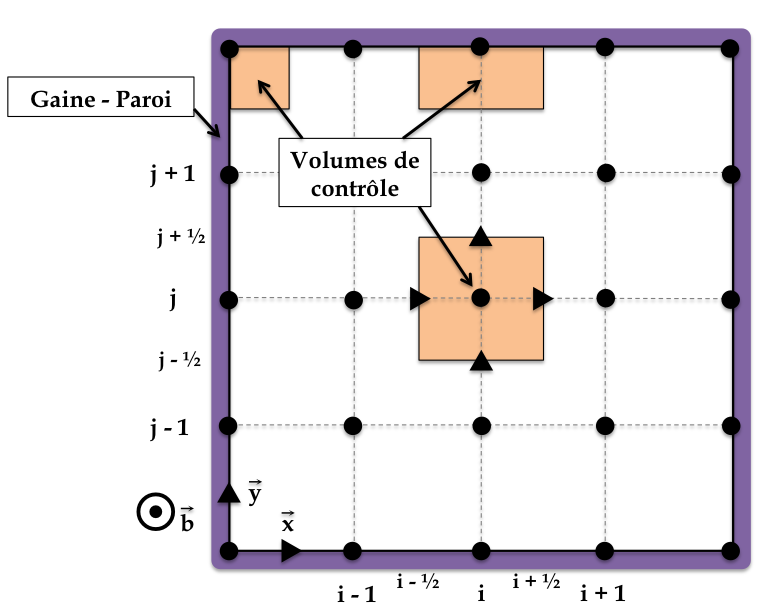
\includegraphics[height=64mm,width=80mm]{figures/3-magnisGrid.png}
{\caption{Schéma du domaine du simulation, entouré d'une gaine
non-collisionnelle.
Les quantités scalaires $n$, $\Phi$ et $T_e$ sont définies aux noeuds et sur les
bords du maillage. Les composantes x et y des champs vectoriels sont
situées entre les noeuds, sur les arêtes des volumes de contrôle, respectivement
au niveau des flêches horizontales et verticales.}
\label{3-maillage}}
\end{figure}

Pour résoudre les systèmes linéaires du modèle, nous utilisons un solveur
9-points développé au GREPHE par Gerjan Hagelaar qui se base sur la procédure
MSI (Modified Strongly Implicit Procedure) décrite par Schneider
dans~\parencite{Schneider} et qui tient compte du caractère intrinsèquement lié
des équations fluides pour diminuer le nombre d'itération nécéssaire pour
trouver la solution du problème. Autorisant des conditions aux limites
périodique, le solveur est de plus construit pour utiliser une approche multi-grille
rendant la convergence particulièremant rapide sur un maillage 2D.

\subsection{Fréquences, termes sources et conditions parallèles}
Avant de résoudre à proprement dit les équations du modèle, MAGNIS
calcule l'ensemble des fréquences. En présence de plusieurs espèces, la
fréquence effective, résultat de toutes les interactions, s'écrit :

\begin{equation*}
\nu_{\alpha}=n_\alpha\sum_{s\neq\alpha} \frac{m_s}{m_\alpha+m_s}
n_sk^m_{\alpha s}
\end{equation*}

A chaque itération, les coefficients $k^m_{\alpha s}=\left<\sigma^m_{\alpha
s}v_r\right>$, où $\sigma^m_{\alpha
s}$ est la section efficace de l'interaction et $v_r$ la vitesse relative des
particules en collision, sont lus dans des tables en fonction de l'énergie des
particules.
Les valeurs des sections efficaces et des coefficients contenus dans ces tables
sont issues de LXCAT~\parencite{LXCAT}, calculées par des expériences de
swarm~\parencite{Phelps} ou encore obtenues en résolvant directement l'équation
de Boltzmann~\parencite{Bolsig}. Un grand
nombre de réactions chimiques peuvent éventuellement être prises en compte.
Dans le cas d'un plasma n'étant constitué que d'une seule espèce, l'ensemble
de fréquences se réduit à la fréquence de collision électrons-neutres
$\nu_{en}$, ions-neutres $\nu_{in}$ et d'ionisation $\nu_\text{iz}$.

Le terme source de particule est calculé en fonction de la fréquence
d'ionisation :
\begin{equation*}
\mathcal{S}_{\alpha}=n_\alpha n_g
k^m_{\alpha_\text{iz}}(T_e)=n_\alpha\nu_{\alpha_\text{iz}}
\end{equation*}

Le terme de perte d'énergie par électron, $\Pi$, est lui aussi fortement
dépendant de la température électronique. Afin de résoudre correctement
l'évolution de la température, le terme est décomposé par une itération
de Newton\footnote{Cette technique peut être utilisée en toute généralité pour
renforcer la stabilité numérique en présence de pertes lorsque celles-ci
dépendent fortement de la quantité perdue 
$\frac{d\mathcal L}{d\mathcal Q}<0$.
La perte est alors décomposée suivant une itération de Newton pour renforcer son
influence :
\begin{equation*}
\mathcal L^{k+1}=\mathcal L^{k}+\frac{d\mathcal L^{k}}{d\mathcal Q}(\mathcal
Q^{k+1}-\mathcal Q^k) \end{equation*}
Originalement mise en \oe vre dans les travaux de
Hagelaar~\parencite{HagelaarImpl}, nous utilisons cette technique pour quelques
termes du modèle.} :
\begin{equation*}
en_e\Pi(T_e^{k+1})=en_e\left(\Pi(T_e^{k})+\frac{\partial\Pi}{\partial
T_e}\left(T_e^{k+1}-T_e^{k}\right)\right)= en_en_g\left(k_{\varepsilon}+
\frac{\partial k_{\varepsilon}}{\partial T_e}(T_e^{k+1}-T_e^{k})\right)
\end{equation*}

avec $k_\varepsilon$ un coefficient de transfert d'énergie (sommé sur 
l'ensemble des processus de collision).

Enfin, les vitesses des particules au niveau des parois sont calculées en
fonction de leur nature isolante, conductrice ou polarisée (les expressions
sont données dans \ref{3-vitessesBord}) puis prisent en compte implicitement
dans les équations de continuité.

\subsection{Expression des vitesses et conservation du courant}
L'un des points clés du modèle tient à la méthode de résolution de l'équation du
mouvement et de la conservation du courant. Ecrivons \eqref{3-eqMouvement} comme
une équation algébrique d'inconnue $\mathbf u$, reliant la fréquence caractéristique du transport
$\omega\sim\partial_t$, une fréquence de collision effective $\nu_m$ et la
fréquence cyclotronique $\omega_c$ avec un champ
accélérateur $\mathbf F$ incluant le terme inertiel d'advection :

\begin{equation}
\label{3-eqMvt}
\alpha_\omega\partial_t \mathbf{u} + 
\nu_m\mathbf{u}+\omega_{c}\mathbf{b}\times\mathbf{u}=
\mathbf F
\end{equation}

avec 
\begin{equation*}\mathbf F=\frac{q}{m}E-\frac{e\nabla
n T}{m
n}-\alpha_u\mathbf{u}\cdot\nabla\mathbf{u}
\end{equation*}

Les facteurs $\alpha_\omega$ et $\alpha_u$ sont des paramètres numériques qui
permettent de modifier l'influence des termes d'inertie, ou éventuellement de
les négliger ($\alpha_{\omega,u}$=0). Discrétisons temporellement
\eqref{3-eqMvt} en prenant la vitesse implicitement dans les termes
magnétique et collisionnel\footnote{Une récente modification permet de choisir
une résolution implicite du terme
d'inertie $\mathbf{u}\cdot\nabla\mathbf{u}$, rendant le code MAGNIS
full-implicit. Cependant dans ce document, pour des raisons de lisibilité, nous
le laisserons inclus dans la force $\mathbf F$.} :

\begin{equation}
\label{3-eqMvtDiscretT}
\delta\left(\mathbf{u}^{k+1}-\mathbf{u}^{k}\right) + 
\nu_m\mathbf{u}^{k+1}+\omega_{c}\mathbf{b}\times\mathbf{u}^{k+1}=
\mathbf F
\end{equation}

où $\delta=\alpha_\omega/\Delta t$. En combinant \ref{3-eqMvtDiscretT} et
l'expression de son produit vectoriel par $\mathbf b$, on peut éliminer le
terme de Laplace. La vitesse s'exprime alors comme une somme pondérée du
transport perpendiculaire et du transport croisé :
\begin{equation}
\label{3-eqMvtPonderee}
\mathbf{u}^{k+1}=A\left(\mathbf F + \delta\mathbf{u}^{k}\right)+ B\mathbf
b\times\left(\mathbf F + \delta\mathbf{u}^{k}\right)
\end{equation}
avec 
\begin{equation*}
\label{3-coefficientsVitesses}
A=\frac{\nu_m+\delta}{(\nu_m+\delta)^2+\omega_c^2}\;\;\;\;\text{et}\;\;\;B=-\frac{\omega_c}{(\nu_m+\delta)^2+\omega_c^2}
\end{equation*}

L'expression ainsi obtenue pour la vitesse
fluide fait intervenir le champ électrique à travers le terme $\mathbf F$.
L'évaluation de ce terme avec un champ électrique pris au temps $k$+1 peut alors
s'écrire en fonction du changement de potentiel :

\begin{equation}
\label{3-eqCorrection}
\mathbf F(\mathbf E^{k+1}) = \mathbf F(\mathbf E^{k})-\frac{q}{m}\nabla
(\Phi^{k+1}-\Phi^{k})
\end{equation}

Cette propriété est ensuite mise à profit afin d'utiliser une méthode de
prédiction-correction pour les vitesses fluides. Celles-ci sont calculées
explicitement dans une première étape à partir de l'ancien champ électrique,
puis corrigées par le changement de potentiel
$\Theta=q(\Phi^{k+1}-\Phi^k)/m$ :

\begin{equation}
\label{3-eqCorrectionVitesse}
\mathbf u^{k+1} = \tilde{\mathbf u}^{k+1}-A\nabla
\Theta-B\mathbf b\times\nabla
\Theta
\end{equation}

Pour résoudre la différence de potentiel, on considère l'équation de
conservation du courant~\eqrefp{eqCourant} dans laquelle on substitue les
vitesses par leur expression (données par \eqref{3-eqCorrectionVitesse}) :

\begin{equation}
\begin{split}
\label{3-eqCourantCoefficient}
\nabla\cdot(-(\sum_iq_in_iA_i-en_eA_e)\nabla
\Theta-(\sum_iq_in_iB_i-en_eB_e)\mathbf
b\times\nabla
\Theta)\\=(en_e\tilde{\mathbf
u}_e^{k+1}-\sum_iq_in_i\tilde{\mathbf u}_i^{k+1})-\mathcal L_{j_\para}
\end{split}
\end{equation}

Après cette correction, l'ensemble des vitesses fluides $\mathbf u_\alpha$
satisfait exactement à la continuité du courant. 

\subsubsection{Sous-relaxation et maillages croisés}
L'équation \eqref{3-eqCourantCoefficient}, discrétisée spatialement sur un
stencil à 9 points, mène à un système linéaire potentiellement mal conditionné
quand le coefficient $B$ devient supérieur au coefficient $A$, ie. en présence
d'un fort champ magnétique. Pour nous assurer que $A>B$ en toutes circonstances,
l'une des solutions est de choisir un pas de temps inférieur à l'inverse de la
fréquence cyclotronique $\Delta t\leq\omega_{ce}\puissance{-1}$ et
ainsi résoudre l'intégralité du mouvement électronique. Cependant, du fait de la
très faible masse des électrons, on peut s'attendre à ce que les termes
d'inertie ne jouent pas un très grand rôle macroscopiquement et qu'une
description des fréquences de l'ordre de $\omega_{ce}$ soit inutile.

Il est aussi possible d'augmenter artificiellement la valeur de $A$ en
remplaçant le facteur $\delta$ par :

\begin{equation*}
\delta=\max(\alpha_\omega/\Delta t,|\omega_c|)
\end{equation*}

Cette opération, qui n'a objectivement aucun effet pour les
ions\footnote{Dans des champs magnétiques typiquement de l'ordre de la centaine
de Gauss, le pas de temps choisit, de l'ordre de 10$^{-8}$s, est toujours bien
inférieur à l'inverse des fréquences cyclotroniques ioniques.}, permet de
sous-relaxer la vitesse électronique à l'échelle cyclotronique. En nous assurant
que celle-ci n'évolue pas trop brutalement, le pas de temps peut alors être
largement augmenté sans modification significative des solutions\footnote{Cette
technique semble néanmoins avoir un impact négatif quand la résolution spatiale
dépasse une certaine échelle, faisant apparaître des structures dont la taille
peut varier en fonction du maillage... Nous cherchons encore à
expliquer ce phénomène et à quantifier le seuil de validité de la technique,
l'augmentation artificielle du terme d'inertie (correspondant à une augmentation
de la masse électronique) pouvant amener une modification des fréquences
hybrides qui entrent en jeu dans l'évolution acoustique du plasma.}.

Sur cette sous-relaxation, l'interpolation nécéssaire à l'évaluation du
membre de droite dans \eqref{3-eqCourantCoefficient} mène inexorablement à l'introduction d'une
erreur dans l'évolution de la vitesse. Au bout de quelques $\Delta t$, cette
erreur peut se propager à l'ensemble des points et s'accumuler,
entraînant de sérieux problèmes de convergence à petit pas de temps. Pour remédier à ce problème, nous
limitons l'erreur d'interpolation en suivant à la fois la vitesse
et la vitesse croisée sur tous les points du maillage :

\begin{equation}
\label{3-eqMvtPonderee}
\mathbf{u}^{k+1}=A\left(\mathbf F + \delta\mathbf{u}^{k}\right)+ B\left(\mathbf
b\times\mathbf F +
\delta\left((1-\beta)\mathbf{u}_\times^{k}+\beta\mathbf
b\times\mathbf{u}^{k}\right)\right)
\end{equation}
\begin{equation}
\label{3-eqMvtPonderee}
\mathbf{u}_\times^{k+1}=-B\left(\mathbf F + \delta\mathbf{u}^{k}\right)+
A\left(\mathbf
b\times\mathbf F +
\delta\left((1-\beta)\mathbf{u}_\times^{k}+\beta\mathbf
b\times\mathbf{u}^{k}\right)\right)
\end{equation}

Le coefficient $\beta$ est un paramètre donnant un contrôle sur
l'utilisation de ce maillage secondaire. Quand $\beta$=0, aucune
interpolation n'est nécéssaire, mais $\mathbf{u}$ et $\mathbf{u}_\times$
tendent à se désynchroniser et le schéma numérique diverge vite. Il faut en
fait un minimum d'interpolation $\beta$>0 pour garder les vitesses consistantes entre elles
(tout en gardant en tête que trop d'interpolation $\beta\rightarrow$1 mène à une
explosion de l'erreur à petit pas de temps). Un calcul analytique pour estimer
l'erreur d'interpolation montre qu'un choix approprié pour le paramètre $\beta$
est :

\begin{equation}
\label{3-eqMvtPonderee}
\beta=\left(\frac{\nu^2+\omega_c^2}{(\delta+\nu)^2+\omega_c^2}\right)^{1/2}
\end{equation}

avec cette valeur, le schéma numérique converge proprement pour n'importe quel
ordering entre $\nu$, $\omega_c$ et $\delta$.

\subsection{Equations de continuité ioniques}
Les équations de continuité pour les espèces ioniques sont résolues avec les
vitesses $\mathbf u_i^{k+1}$, en utilisant au choix un schéma
Upwind-explicite/implicite ou MUSCL-explicite/implicite :

\begin{equation}
n_i^{k+1}+\nabla\cdot(n_i^{k/k+1}\mathbf u_i^{k+1})=\mathcal S_i-\mathcal
L_{i_\para}
\end{equation}

Les pertes parallèles $L_{i_\para}$ et aux bords du
domaines sont implicitées afin de s'assurer que la densité ne devienne pas
négative.

\subsection{Flux de chaleur et équation d'énergie}

Le flux de chaleur porté par les électrons étant sensible au champ magnétique de
la même façon que le flux de particules, nous adoptons la même méthode que
précédemment. Le flux de chaleur est tout d'abord prédit en fonction de
l'ancien gradient de température :
\begin{equation}
\label{3-eqChaleurPonderee}
\tilde{\mathbf{q}}_e^{k+1}=-A_e(
\frac{5e^2n_eT_e}{2m_e}\nabla T_e^k+\delta q_e^k)-B_e\mathbf
b\times(\frac{5e^2n_eT_e}{2m_e}\nabla T_e^k +\delta q_e^k)
\end{equation}

avec les mêmes coefficients $A_e$ et $B_e$ que pour le flux électronique. On
corrige ensuite le flux de chaleur en prenant en compte sa réponse au changement
de température $\mathcal T=e(T_e^{k+1}-T_e^k)$ :

\begin{equation}
\label{3-eqCorrectionVitesse}
\mathbf q^{k+1} = \tilde{\mathbf q}^{k+1}-A_\varepsilon\nabla
\mathcal T+B_\varepsilon\mathbf b\times\nabla
\mathcal T
\end{equation}

avec 
\begin{equation*}
\label{3-coefficientsChaleur}
A_\varepsilon=A_e\frac{5en_eT_e}{2m_e}\;\;\;\;\text{et}\;\;\;B_\varepsilon=B_e\frac{5en_eT_e}{2m_e}
\end{equation*}

L'équation d'énergie \eqref{3-eqTemperature} est utilisée pour résoudre le
changement de température $\mathcal T$. 

\begin{equation}
\label{3-eqTemperature2}
\begin{split}
\left(\frac{3n_e}{2\Delta
t}+n_e\frac{\partial\Pi}{\partial T_e}+\max(C,0)\right)\mathcal T
-\nabla\cdot\left(A_\varepsilon\nabla\mathcal T- B_\varepsilon\mathbf
b\times\nabla\mathcal T\right)\\ =  C eT_e^k -\nabla\tilde{\mathbf q}_e^{k+1}+
en_e(\mathcal{P}_\text{ext}-\Pi)-\mathcal L_{\varepsilon_\para}
\end{split}\end{equation}

avec 

\begin{equation*}C=-\frac{5}{2}\mathcal S_e-\frac{3}{2}n_e\mathbf
u_e\frac{\nabla
T_e^k}{T_e^k}+(2n_e\nu_e+\mathcal{S}_e)\frac{\mathcal{U}_e}{eT_e^k} +\frac{\text{d} n_e}{\text{d} t}
\end{equation*}

Le coefficient $C$ contient les termes qui peuvent apporter une contribution
négative dans l'équation d'énergie. Si l'un des
termes de $C$ est positif, nous le décomposons suivant une itération de
Newton en le supposant proportionnel à $T_e$. Le terme est alors comptabilisé
implicitement, stabilisant et accélérant la convergence du schéma
\parencite{HagelaarImpl} :

\begin{equation*}
	C<0\rightarrow C^{k+1}=C^{k}+\frac{\partial C^k/T_e\,T_e}{\partial
	T_e}(T_e^{k+1}-T_e^k)=C^{k}+ C^k/T_e^k\mathcal T
\end{equation*}

\subsection{Etude de convergence sur maillage} 
Afin de vérifier le schéma numérique de MAGNIS, nous réalisons dans ce
paragraphe une étude de convergence sur maillage. 

Le cas de test correspond à une configuration magnétique complexe de type filtre
dans un plasma d'argon avec des parois conductrices. L'intensité du
champ magnétique est choisie suffisament importante $B$=250 G pour
tester le modèle dans une situation assez défavorable. La pression est prise à 100 mTorr
pour supprimer les phénomènes non stationnaires qui apparaissent à basse
pression et qui rendent impossible cette étude.

La figure~\ref{3-convergence} montre l'erreur relative calculée pour la densité
totale du plasma à l'état stationnaire. On voit que l'erreur décroît comme le carré
de l'inverse du nombre de maille, donnant un ordre 2 pour la convergence du
schéma de MAGNIS.

\begin{figure}[htbp]
\centering
\includegraphics[height=70mm]{figures/3-convergence.eps}
{\caption{Erreur relative des solutions calculées en fonction de l'échelle du
maillage h=1/\#points.}
\label{3-convergence}}
\end{figure}

A partir d'un maillage grossier de taille 16x16, nous construisons une série de
maillages rafinés d'un facteur 2 dans chaque
direction par rapport à leur prédécesseur, la grille la
plus fine de cette étude étant de taille 512x512. Comme nous n'avons pas de
solution analytique au cas de test, nous utilisons l'extrapolation de
Richardson comme solution de référence~\parencite{Roache} :

\begin{equation}
f_{h=0}=\frac{4}{3}f_{1}-\frac{1}{3}f_2
\end{equation}

$f_{1}$ et $f_2$ étant les solutions calculées sur les maillages les plus fins,
ie. respectivement sur 512 et 256 points de maillages. Avec cette solution,
l'erreur relative (mesurée suivant la norme L1) correpondant à un maillage
d'échelle $h$ ($h$ est égal à l'inverse du nombre de points) s'écrit :

\begin{equation}
\epsilon\,(\text{\%})=\frac{|f_h-f_{h=0}|}{f_{h=0}}
\end{equation}

Bien que d'autres
vérifications comme la convergence temporelle, la méthode des solutions manufacturées, ou
une étude des taux de croissance des modes du système n'aient pas été
entreprises, celles-ci seront les bienvenues pour tester davantage les
solutions calculées par MAGNIS. La validation du code est quant à elle réalisée
dans le chapitre suivant, à travers trois études de cas simplifiées
représentatives d'expérimentations réelles.



%\bibliographystyle{alpha}
%\bibliography{biblio}
\end{refsection}

